% Options for packages loaded elsewhere
\PassOptionsToPackage{unicode}{hyperref}
\PassOptionsToPackage{hyphens}{url}
%
\documentclass[
]{article}
\title{HCM SCD risk algorithm cost-effectiveness analysis}
\author{Nathan Green, UCL \and Yang Chen, UCL}
\date{2022-02-15}

\usepackage{amsmath,amssymb}
\usepackage{lmodern}
\usepackage{iftex}
\ifPDFTeX
  \usepackage[T1]{fontenc}
  \usepackage[utf8]{inputenc}
  \usepackage{textcomp} % provide euro and other symbols
\else % if luatex or xetex
  \usepackage{unicode-math}
  \defaultfontfeatures{Scale=MatchLowercase}
  \defaultfontfeatures[\rmfamily]{Ligatures=TeX,Scale=1}
\fi
% Use upquote if available, for straight quotes in verbatim environments
\IfFileExists{upquote.sty}{\usepackage{upquote}}{}
\IfFileExists{microtype.sty}{% use microtype if available
  \usepackage[]{microtype}
  \UseMicrotypeSet[protrusion]{basicmath} % disable protrusion for tt fonts
}{}
\makeatletter
\@ifundefined{KOMAClassName}{% if non-KOMA class
  \IfFileExists{parskip.sty}{%
    \usepackage{parskip}
  }{% else
    \setlength{\parindent}{0pt}
    \setlength{\parskip}{6pt plus 2pt minus 1pt}}
}{% if KOMA class
  \KOMAoptions{parskip=half}}
\makeatother
\usepackage{xcolor}
\IfFileExists{xurl.sty}{\usepackage{xurl}}{} % add URL line breaks if available
\IfFileExists{bookmark.sty}{\usepackage{bookmark}}{\usepackage{hyperref}}
\hypersetup{
  pdftitle={HCM SCD risk algorithm cost-effectiveness analysis},
  pdfauthor={Nathan Green, UCL; Yang Chen, UCL},
  hidelinks,
  pdfcreator={LaTeX via pandoc}}
\urlstyle{same} % disable monospaced font for URLs
\usepackage[margin=1in]{geometry}
\usepackage{longtable,booktabs,array}
\usepackage{calc} % for calculating minipage widths
% Correct order of tables after \paragraph or \subparagraph
\usepackage{etoolbox}
\makeatletter
\patchcmd\longtable{\par}{\if@noskipsec\mbox{}\fi\par}{}{}
\makeatother
% Allow footnotes in longtable head/foot
\IfFileExists{footnotehyper.sty}{\usepackage{footnotehyper}}{\usepackage{footnote}}
\makesavenoteenv{longtable}
\usepackage{graphicx}
\makeatletter
\def\maxwidth{\ifdim\Gin@nat@width>\linewidth\linewidth\else\Gin@nat@width\fi}
\def\maxheight{\ifdim\Gin@nat@height>\textheight\textheight\else\Gin@nat@height\fi}
\makeatother
% Scale images if necessary, so that they will not overflow the page
% margins by default, and it is still possible to overwrite the defaults
% using explicit options in \includegraphics[width, height, ...]{}
\setkeys{Gin}{width=\maxwidth,height=\maxheight,keepaspectratio}
% Set default figure placement to htbp
\makeatletter
\def\fps@figure{htbp}
\makeatother
\setlength{\emergencystretch}{3em} % prevent overfull lines
\providecommand{\tightlist}{%
  \setlength{\itemsep}{0pt}\setlength{\parskip}{0pt}}
\setcounter{secnumdepth}{-\maxdimen} % remove section numbering
\newlength{\cslhangindent}
\setlength{\cslhangindent}{1.5em}
\newlength{\csllabelwidth}
\setlength{\csllabelwidth}{3em}
\newlength{\cslentryspacingunit} % times entry-spacing
\setlength{\cslentryspacingunit}{\parskip}
\newenvironment{CSLReferences}[2] % #1 hanging-ident, #2 entry spacing
 {% don't indent paragraphs
  \setlength{\parindent}{0pt}
  % turn on hanging indent if param 1 is 1
  \ifodd #1
  \let\oldpar\par
  \def\par{\hangindent=\cslhangindent\oldpar}
  \fi
  % set entry spacing
  \setlength{\parskip}{#2\cslentryspacingunit}
 }%
 {}
\usepackage{calc}
\newcommand{\CSLBlock}[1]{#1\hfill\break}
\newcommand{\CSLLeftMargin}[1]{\parbox[t]{\csllabelwidth}{#1}}
\newcommand{\CSLRightInline}[1]{\parbox[t]{\linewidth - \csllabelwidth}{#1}\break}
\newcommand{\CSLIndent}[1]{\hspace{\cslhangindent}#1}
\ifLuaTeX
  \usepackage{selnolig}  % disable illegal ligatures
\fi

\begin{document}
\maketitle

\hypertarget{introduction}{%
\section{Introduction}\label{introduction}}

Hypertrophic cardiomyopathy (HCM) is a common inherited heart muscle
disorder and a leading cause of sudden cardiac death (SCD) in young
adults. Patients at high risk of SCD need to be identified so they can
be offered lifesaving treatment with an implantable cardioverter
defibrillator (ICD). Contemporary guidelines recommend that the sudden
death risk is assessed by evaluating clinical parameters that reflect
the severity of the underlying myocardial disease. The presence or
absence of these risk factors is then used to guide clinical
decision-making with respect to prophylactic ICD implantation. Although
observational cohort studies show that this approach identifies patients
with the greatest risk of SCD, validation of current algorithms suggests
that they overestimate risk, resulting in inappropriate prophylactic ICD
implantation in a substantial number of patients. A previous study
derived a new sudden death risk model that can be used to generate
individualized risk estimates for SCD and improve the targeting of ICD
therapy in patients with HCM (O'Mahony et al. 2014).

This stated improvement was in terms of reducing the number of patients
who are offered an ICD unnecessarily i.e.~without a shock in their
lifetime, or `false positives'. However, this does not take into account
a more detailed picture which would inform decision-making. The welfare
or health impact on an individual of an ICD and the costs of various
decisions and outcomes.

This is especially timely given new data on real world ICD practice
which shows significant variation across healthcare systems (Nauffal et
al. 2021) and the rise of the s-ICD technology (Lambiase et al. 2022).

This paper addresses the notable gap in the current literature. We will
present cost-effectiveness analyses according to a range of ICD
implantation rates, reflecting differences in real world practice across
geographies. We will also highlight limitations to the health economic
model and the fragility of conclusions drawn based on a range of
sensitivity analyses.

All code is made publicly available on GitHub at
www.github/n8thangreen/hcm\_scd\_cemodel/.

EDIT ``For primary prevention, the cost-effectiveness of ICD has been
widely studied, but uncertainty about its cost-effectiveness remains.
The cost-effectiveness ratios vary between studies depending on the
patient characteristics, methodology, perspective, and national
settings. Among the European studies, the conclusions are varied, where
the ICD is considered cost-effective or not dependent on the study''

\hypertarget{previous-work}{%
\subsection{Previous work}\label{previous-work}}

There have been previous cost-effectiveness analyses of ICD implants
(Magnusson and Wimo 2020; Cowie et al. 2009; Mealing et al. 2016; Smith
et al. 2013)

(Yao et al. 2007) use a Markov model and consider multiple implantation
attempts if unsuccessful. (Colquitt et al. 2014) is a Health Technology
Assessment which compares optimal pharmacological therapy (OPT) with or
without ICD. (Tomini 2016) is a review of economic evaluation models for
cardiac resynchronization therapy with implantable cardioverter
defibrillators in patients with heart failure. (Ommen et al. 2020) 2020
AHA/ACC Guideline for the Diagnosis and Treatment of Patients With
Hypertrophic Cardiomyopathy.

(O'Mahony et al. 2014) provided a systematic review and meta-analysis.
Using 7000 unselected patients with HCM from Europe, Asia, Middle East,
North and South America, main findings support the 2014 ESC guideline
recommendations for the primary prevention of SCD. Pooled prevalence of
SCD endpoints was 1.0\% (95\% CI 0.52 to 1.61) in low-risk patients
(\textless4\% over 5 years), 2.43 (95\% CI 1.23 to 3.92) in
intermediate-risk patients (4-6\% in 5 years) and 8.39 (95\% CI 6.68 to
10.25) in high-risk patients (\textgreater6\% in 5 years).

Compared with data analyses of the same cohort (\textbf{Lorenzini2019?})
\(N=4800\), {[}hypertrophic cardiomyopathy outcome investigators
cohort{]} The main survival analysis was based on a composite end point
consisting of all-cause mortality, aborted SCD, and heart transplant.
After a median follow-up of 6.2 years (IQR, 3.1-9.8), 721 patients
(14.7\%) reached the composite study end point. 3.4\% met the SCD or
equivalent end point (SCD, 138 {[}2.8\%{]}; aborted SCD, 30
{[}0.6\%{]}); 2.2\% died of other CV causes; 212 patients (4.3\%) died
of non-CV causes.

Main cause of death in younger patients was SCD (or equivalent), but
this accounted for a progressively smaller percentage of total deaths
with advancing age, whereas HF death or cardiac transplantation
accounted for a similar proportion of events throughout the age
spectrum. Female patients had higher excess mortality than male patients
did (SMR, 2.66; 95\% CI, 2.38-2.97 vs SMR, 1.68; 95\% CI, 1.52-1.85; P
\textless{} .001) and female sex was independently associated with a
worse prognosis after adjusting for baseline differences in a
multivariate model (hazard ratio, 1.28; 95\% CI, 1.09-1.49; P = 0.003).

\textbf{Comparison with other models} (Magnusson and Wimo 2020) Of 1000
simulated patients, after 12 years, 402 lives were saved. QALYs were
derived from the Swedish tariff of EQ5D-3L for people at age 50--75
years. It is assumed that people with HCM have lower utilities than in
the general population (multiplied by 0.8).

(Smith et al. 2013) Lifetime horizon, non HCM ICD cohort. Lifetime
horizon but monthly cycles! Netherlands registry used. They quote
(Sanders, Hlatky, and Owens 2005) for the 0.88 utility.

(Cowie et al. 2009) -\textgreater{} Non-HCM population. Mean age once
more in late 50s. They modify Sanders model by incorporating Belgian
life tables to adjust the non cardiac mortality rate, and define
specific categories of death.

(Mealing et al. 2016) -\textgreater{} Lifetime horizon, Non HCM ICD
cohort. Starting age 66. References NIHR (Buxton et al. 2006). Good
supplemental appendix

(Thijssen et al. 2014) -- monthly cycle, lifetime horizon non HCM
cohort.

(García-Pérez et al. 2015) -- Systematic review of cost effectiveness of
ICD, of 18 studies identified for primarr prevention cohort, 7 purely
ischaemic aetiology, others mixed. Overall v low HCM numbers. All 2010
and before. (Bryant et al. 2007) appears to be an older version of
Garcia Perez

(Caro et al. 2007) -\textgreater{} cost benefit analyses

\hypertarget{data}{%
\section{Data}\label{data}}

The data set has been described in detail elsewhere (see (O'Mahony et
al. 2014)) so we will describe it briefly here. The main data set
contains \(n\) = 3672 individuals follow-up data of patients with HCM
who may have been given an ICD depending on clinical and patient
factors.

Key cohort characteristics include the following. Patients were enrolled
from the 6 health centres: Athens (474), Bologna (456), Coruna (590),
London (1592), Murcia (404), Naples (156); The number of uncensored
individuals was 197 (5\%); The mean age (sd) was 48(16); The start of
study data collection was in 1972 to 2011. Further plots are given in
the Appendix.

Health and cost data were obtained from literature and expert opinion.
Table 1 presents the unit cost and health values used in the model.

\begin{longtable}[]{@{}
  >{\raggedright\arraybackslash}p{(\columnwidth - 8\tabcolsep) * \real{0.38}}
  >{\raggedright\arraybackslash}p{(\columnwidth - 8\tabcolsep) * \real{0.15}}
  >{\raggedright\arraybackslash}p{(\columnwidth - 8\tabcolsep) * \real{0.19}}
  >{\raggedright\arraybackslash}p{(\columnwidth - 8\tabcolsep) * \real{0.08}}
  >{\raggedright\arraybackslash}p{(\columnwidth - 8\tabcolsep) * \real{0.20}}@{}}
\caption{Model parameter values. All cost are in pounds sterling and
inflated to 2021 value where necessary. \(^*\)either one-off/on state
entry or recurring.}\tabularnewline
\toprule
\begin{minipage}[b]{\linewidth}\raggedright
Description
\end{minipage} & \begin{minipage}[b]{\linewidth}\raggedright
Parameter
\end{minipage} & \begin{minipage}[b]{\linewidth}\raggedright
Value\(^*\)
\end{minipage} & \begin{minipage}[b]{\linewidth}\raggedright
Range
\end{minipage} & \begin{minipage}[b]{\linewidth}\raggedright
Source
\end{minipage} \\
\midrule
\endfirsthead
\toprule
\begin{minipage}[b]{\linewidth}\raggedright
Description
\end{minipage} & \begin{minipage}[b]{\linewidth}\raggedright
Parameter
\end{minipage} & \begin{minipage}[b]{\linewidth}\raggedright
Value\(^*\)
\end{minipage} & \begin{minipage}[b]{\linewidth}\raggedright
Range
\end{minipage} & \begin{minipage}[b]{\linewidth}\raggedright
Source
\end{minipage} \\
\midrule
\endhead
\emph{Health} & & & & \\
HCM without ICD & \texttt{q\_hcm} & 0.88 QALY/year & 0.6, 1 & Sanders,
Hlatky, and Owens (2005) \\
Manage with ICD & \texttt{u\_icd} & 0.9 & 0.8, 1 & Magnusson and Wimo
(2020); Holbrook2020 \\
Death & \texttt{q\_death} & 0 QALY/year & & \\
Implantation procedure utility & \texttt{u\_implant} & -0.048 & -0.096,
0 & Holbrook et al. (2020) \\
Shock utility & \texttt{u\_shock} & 0.875 & & Buxton et al. (2006) \\
& & & & \\
\emph{Cost} & & & & \\
ICD appointment & \texttt{c\_appt} & £145 & & Cardiology Service (WF02A)
Follow Up Attendance - Multi Professional. NHS England (2021) \\
Perform risk score & \texttt{c\_rs} & £0 & & \\
Implant ICD & \texttt{c\_implant} & £4,666 & & EY02B Tariffs \\
Implant complication & \texttt{c\_compl} & £28,857 & & Formula
derived \\
Non-fatal shock with hospitalisation & \texttt{c\_shock} & £22,880 & &
UK Stroke Assoc. \\
Lead infection & \texttt{c\_inf} & £37,116 & & Thijssen et al. (2014) \\
Lead dislodgement & \texttt{c\_dis} & £6,146 & & Thijssen et al.
(2014) \\
HCM without ICD & \texttt{c\_hcm} & 0 & & \\
Sudden cardiac death (SCD) & \texttt{c\_scd} & 0 & & \\
All-cause death & \texttt{c\_death} & 0 & & \\
& & & & \\
\emph{Probabilities} & & & & \\
Initial implant complication & \texttt{p\_compl} & 0.043 & & Cunningham
et al. (2012) \\
Lead infection & \texttt{p\_inf\_init} & 0.02277 & & Thijssen et al.
(2014) \\
lead dislodgement & \texttt{p\_dis\_init} & 0.00828 & & Thijssen et al.
(2014) \\
& & & & \\
Time horizon & \texttt{T} & 12 years & & \\
Annual number of appointments & \texttt{n\_appt} & 2 & & \\
\bottomrule
\end{longtable}

\hypertarget{methods}{%
\section{Methods}\label{methods}}

The individual-level patient data are first stratified in to two groups
for each risk algorithm. The algorithms are ICD given if Cox model risk
score \textgreater{} 6\% or \textgreater{} 4\%: Using the method from
(O'Mahony et al. 2014).

\hypertarget{markov-model}{%
\subsection{Markov model}\label{markov-model}}

Th patient data provide starting state populations for HCM with ICD and
HCM without ICD which will be different for each risk decision rule.
Further, the transition probabilities from these states will differ
because of the case mixes. We assume that shocked patients return to the
HCM ICD state. A diagram of the cohort model is given in Figure
@ref(fig:model).

\begin{figure}

{\centering \includegraphics[width=3.93in]{../../images/model_diagram} 

}

\caption{HCM ICD Markov model diagram. Bold circles represent starting states with and without ICD and dashed circles represent sink states.}\label{fig:model}
\end{figure}

Therefore, the transition matrix is the following.

\[
\begin{pmatrix}
p_{11} & p_{12} & 0 & 0 & p_{15}\\
1 - p_{15} & 0 & 0 & 0 & p_{15}\\
0 & 0 & p_{33} & p_{34} & p_{35}\\
0 & 0 & 0 & 1 & 0\\
0 & 0 & 0 & 0 & 1
\end{pmatrix}
\]

Model assumptions include the following: We assumed that an ICD patient
has 2 annual appointments. All shocks are treated the same in terms of
costs and health impact. Implantation can have complications and the
cost of an implant complication is taken as a weighted sum of infection
and dislodgement cost with values from (Smith et al. 2013). The time
horizon was set at 12 years from time of implant, following (O'Mahony et
al. 2014). The life cycle duration was one year. This was a balance
between temporal fidelity and parsimony and was appropriate given the
scale at which events occur. The full set of equations for calculating
the health and cost values for each intervention are given in the
Appendix.

\hypertarget{transition-probability-inference}{%
\subsection{Transition probability
inference}\label{transition-probability-inference}}

Using the statistical software for Bayesian analysis, WinBUGS (Lunn et
al. 2000) called from R (R Core Team 2021), each derived data set using
each risk algorithm was used to generate posterior samples of transition
probabilities. Details of the formulae for the Bayesian inference is
provided in the Appendix.

\hypertarget{results}{%
\section{Results}\label{results}}

We give results of the model fitting and cost-effectiveness analysis.

\hypertarget{model-fitting}{%
\subsection{Model fitting}\label{model-fitting}}

The data set was stratified in to two subgroups for each intervention.
Table 2 gives the model starting state populations. Uncertainty is
presented for the Cox risk model values. These were obtained by using
the frequentist confidence intervals from the risk score model fit in
(O'Mahony et al. 2014) and simulating a sample of risk scores for each
individual. The proportion of individuals for the observed and Cox model
6\% threshold are similar but this does not necessarily mean that they
are the same case-mix.

\begin{longtable}[]{@{}llll@{}}
\caption{Starting state populations by decision rule.}\tabularnewline
\toprule
Risk rule & State & N (95\% CI) & Proportion (95\% CI) \\
\midrule
\endfirsthead
\toprule
Risk rule & State & N (95\% CI) & Proportion (95\% CI) \\
\midrule
\endhead
Observed & HCM ICD & 559 & 0.15 \\
& HCM & 3113 & 0.85 \\
Cox risk \textgreater4\% & HCM ICD & 1103 (162, 2390) & 0.3 (0.04,
0.65) \\
& HCM & 2569 (1282, 3510) & 0.7 (0.35, 0.96) \\
Cox risk \textgreater6\% & HCM ICD & 542 (61, 1777) & 0.15 (0.02,
0.48) \\
& HCM & 3130 (1895, 3611) & 0.85 (0.52, 0.98) \\
\bottomrule
\end{longtable}

Figures @ref(fig:transhist) gives densities of posterior distributions
for state transition probabilities for groups with and without ICD
implants using each risk decision rule. We see that the chance of
remaining in the HCM state is lower for the ICD patients selected using
the 6\% risk threshold rule relative to the current approach. Also the
chance of SCD or shock and all-cause death are higher. This indicates
that the new method is better at selecting individuals to have an ICD.

\begin{figure}

{\centering \includegraphics[width=1\linewidth]{../../images/post_hist} 

}

\caption{Density curves of posterior distributions for state transition probabilities from the starting state. Red lines are for ICD patients and blue lines are for non-ICD patients. Each row is for a particular decision rule of 4\% and 6\% threshold Cox model risk score and the observed in the data set.}\label{fig:transhist}
\end{figure}

\hypertarget{cost-effectiveness-analysis}{%
\subsection{Cost-effectiveness
analysis}\label{cost-effectiveness-analysis}}

\newpage

\begin{longtable}[]{@{}llllll@{}}
\caption{Cost-effectiveness statistics per enrolled study individual.
The baseline intervention is that observed in the data.}\tabularnewline
\toprule
Strategy & Cost, \(c\) (£) & \(\Delta c\) (£) & QALYs, \(e\) &
\(\Delta e\) & ICER (£/QALY) \\
\midrule
\endfirsthead
\toprule
Strategy & Cost, \(c\) (£) & \(\Delta c\) (£) & QALYs, \(e\) &
\(\Delta e\) & ICER (£/QALY) \\
\midrule
\endhead
Baseline & 8388.98 & & 9.61 & & \\
Cox \textgreater{} 6\% & 7909.41 & -479.57 & 9.65 & 0.04 & -12,285 \\
Cox \textgreater{} 4\% & 16,216 & 7826.78 & 9.66 & 0.05 & 156,463 \\
\bottomrule
\end{longtable}

Table 3 shows the cost-effectiveness mean summary statistics for
baseline intervention of that observed in the data. We see that the 4\%
risk threshold intervention is approximately double the baseline
expected total cost. This is expected because of the greater number of
ICD patients. The expected total QALYs are very similar between
interventions so that the relative cost-effectiveness is driven by the
total costs. The 6\% risk threshold intervention is both cheaper than
the baseline and has marginally better health outcomes. This is the most
cost-effective option with an ICER of 156,463. These conclusions are
confirmed in the cost-effectiveness acceptability curve (CEAC) in Figure
@ref(fig:ceac) and the cost-effectiveness plane in Figure
@ref(fig:ceplane).

\hypertarget{sensitivity-analysis}{%
\subsubsection{Sensitivity analysis}\label{sensitivity-analysis}}

\begin{longtable}[]{@{}rrrrrrrrr@{}}
\caption{Sensitivity analysis input values.}\tabularnewline
\toprule
scenario & q\_hcm & q\_icd & u\_icd & u\_shock & c\_shock & c\_icd &
c\_rscore & c\_appt \\
\midrule
\endfirsthead
\toprule
scenario & q\_hcm & q\_icd & u\_icd & u\_shock & c\_shock & c\_icd &
c\_rscore & c\_appt \\
\midrule
\endhead
1 & 0.88 & 0.88 & -0.05 & -0.5 & 22880 & 4666 & 0 & 145 \\
2 & 0.50 & 0.88 & -0.05 & -0.5 & 22880 & 4666 & 0 & 145 \\
3 & 1.00 & 0.88 & -0.05 & -0.5 & 22880 & 4666 & 0 & 145 \\
4 & 0.88 & 0.50 & -0.05 & -0.5 & 22880 & 4666 & 0 & 145 \\
5 & 0.88 & 1.00 & -0.05 & -0.5 & 22880 & 4666 & 0 & 145 \\
6 & 0.88 & 0.88 & -0.05 & -0.8 & 22880 & 4666 & 0 & 145 \\
7 & 0.88 & 0.88 & -0.05 & -0.2 & 22880 & 4666 & 0 & 145 \\
8 & 1.00 & 0.00 & 0.00 & 0.0 & 0 & 1 & 0 & 0 \\
\bottomrule
\end{longtable}

\begin{longtable}[]{@{}rrrrr@{}}
\toprule
c\_inf & c\_dis & p\_compl & p\_inf\_init & p\_dis\_init \\
\midrule
\endhead
7116.02 & 6146.035 & 0.047 & 0.02277 & 0.00828 \\
7116.02 & 6146.035 & 0.047 & 0.02277 & 0.00828 \\
7116.02 & 6146.035 & 0.047 & 0.02277 & 0.00828 \\
7116.02 & 6146.035 & 0.047 & 0.02277 & 0.00828 \\
7116.02 & 6146.035 & 0.047 & 0.02277 & 0.00828 \\
7116.02 & 6146.035 & 0.047 & 0.02277 & 0.00828 \\
7116.02 & 6146.035 & 0.047 & 0.02277 & 0.00828 \\
0.00 & 0.000 & 0.000 & 0.00000 & 0.00000 \\
\bottomrule
\end{longtable}

\begin{figure}

{\centering 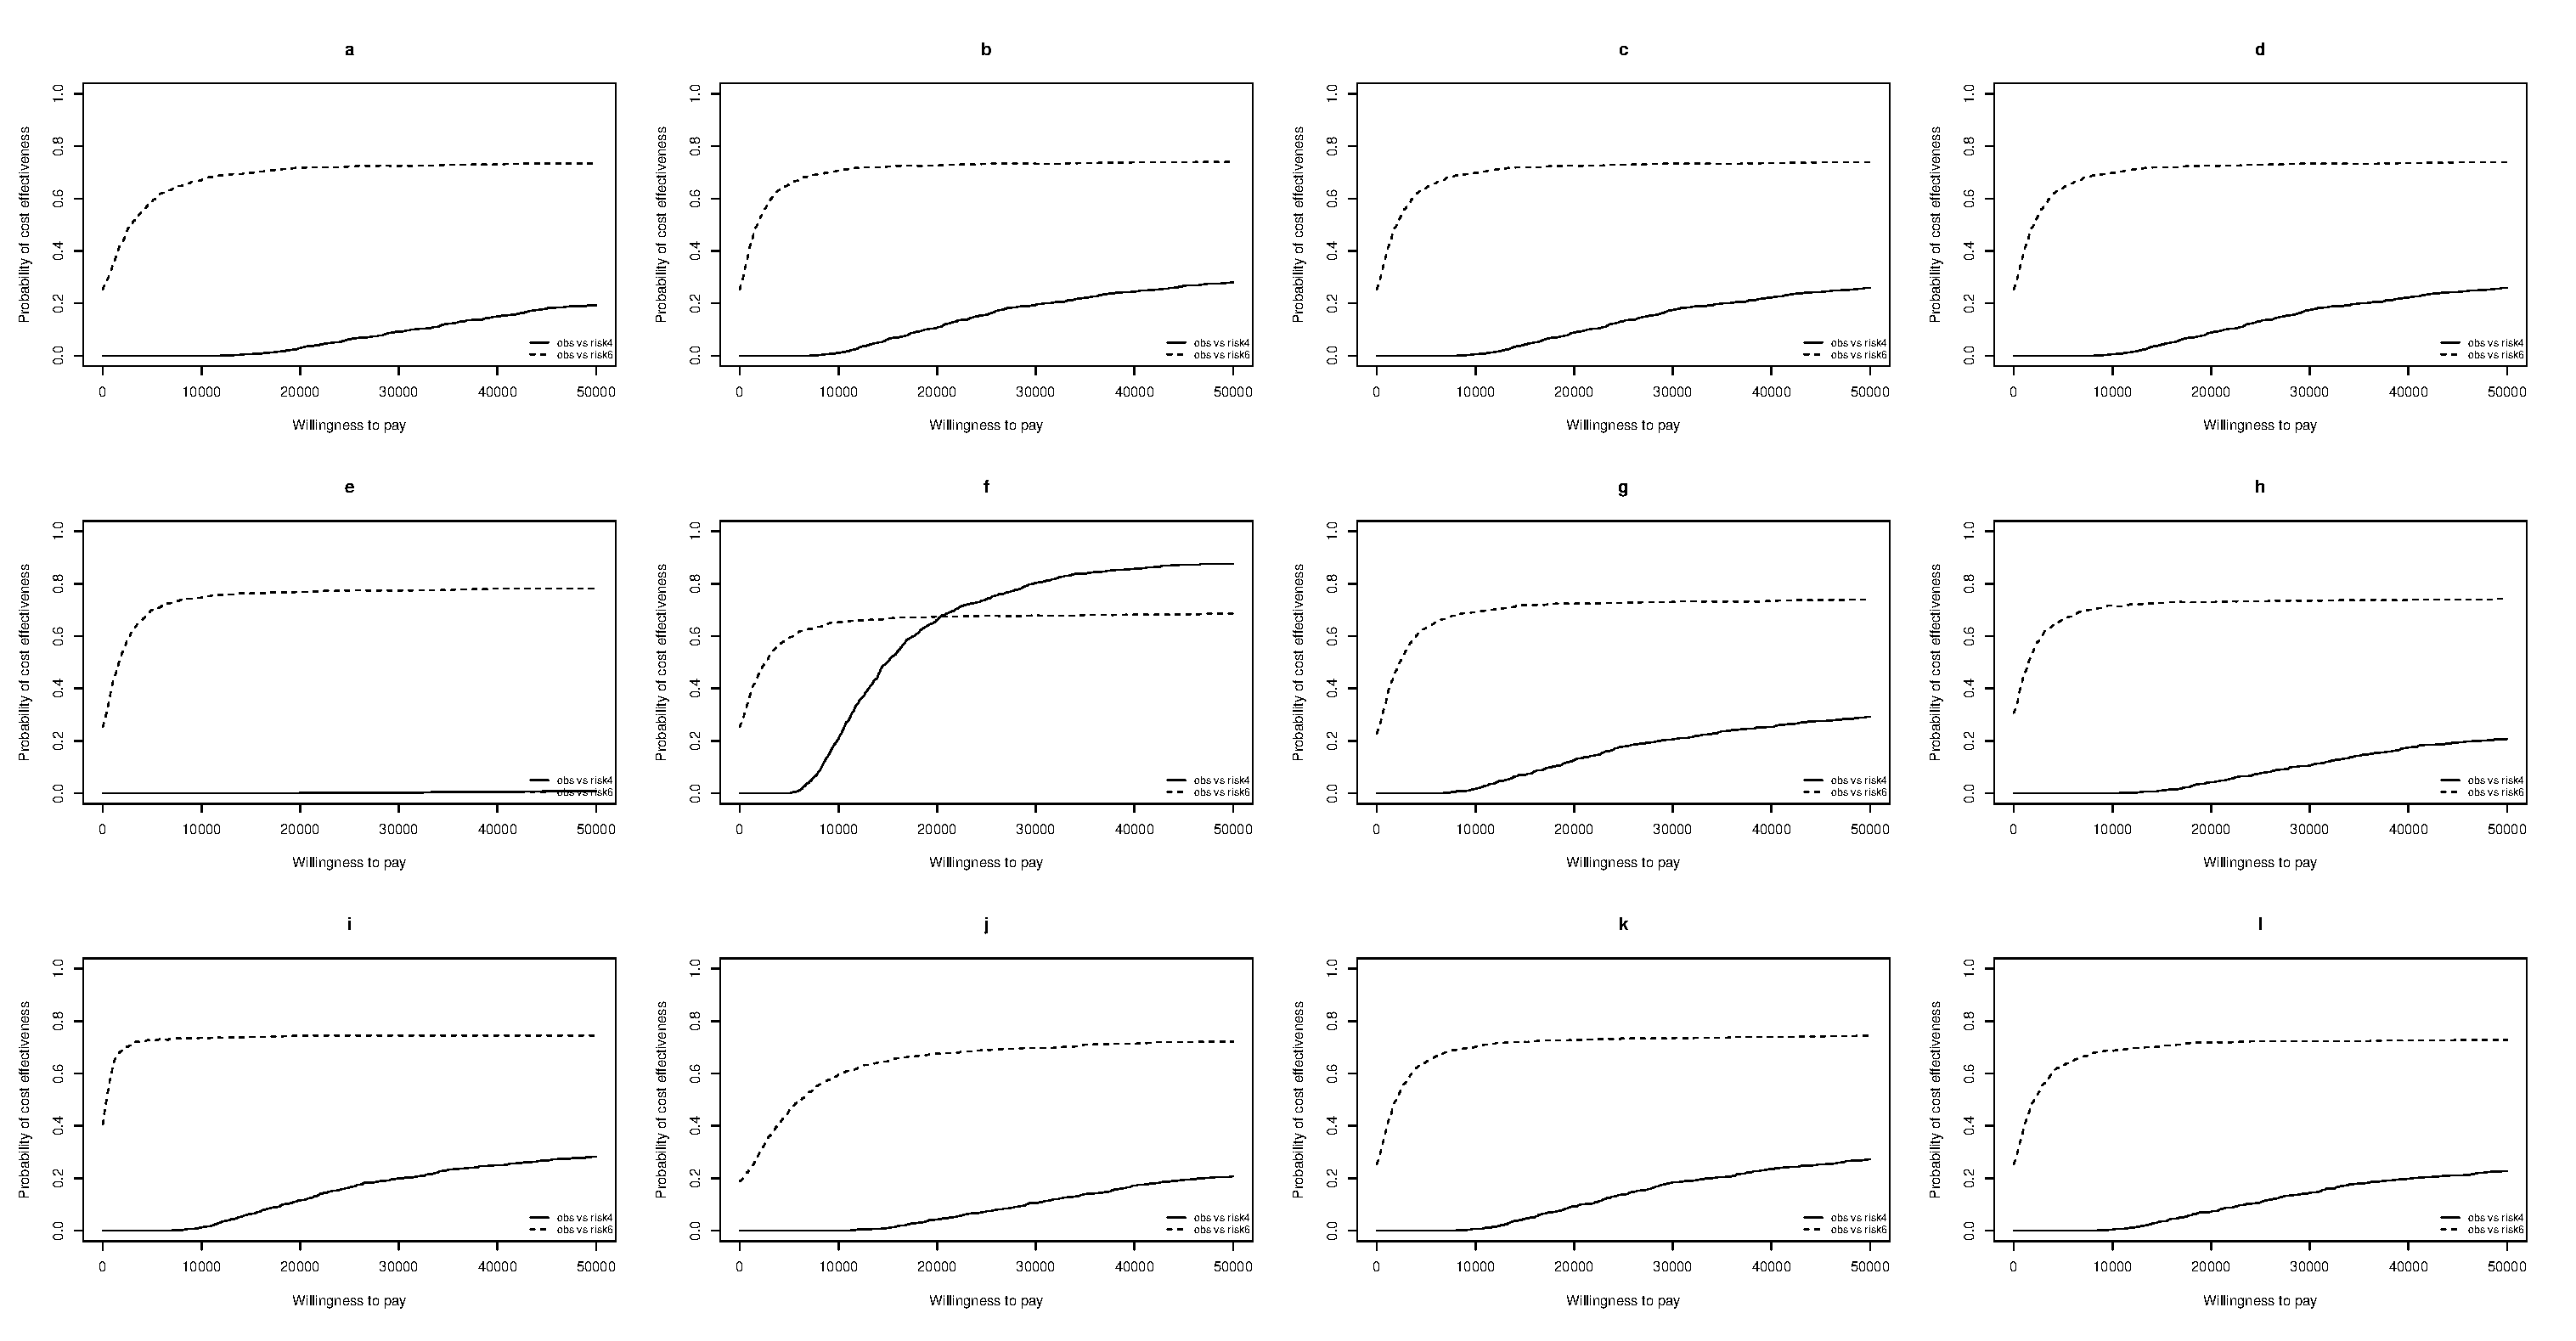
\includegraphics[width=0.6\linewidth]{../../images/ceac_grid} 

}

\caption{Cost-effectiveness acceptability curves (CEAC). Solid line is the 6\% threshold Cox model and dashed line is the 4\% threshold Cox model.}\label{fig:ceac}
\end{figure}

\begin{figure}

{\centering 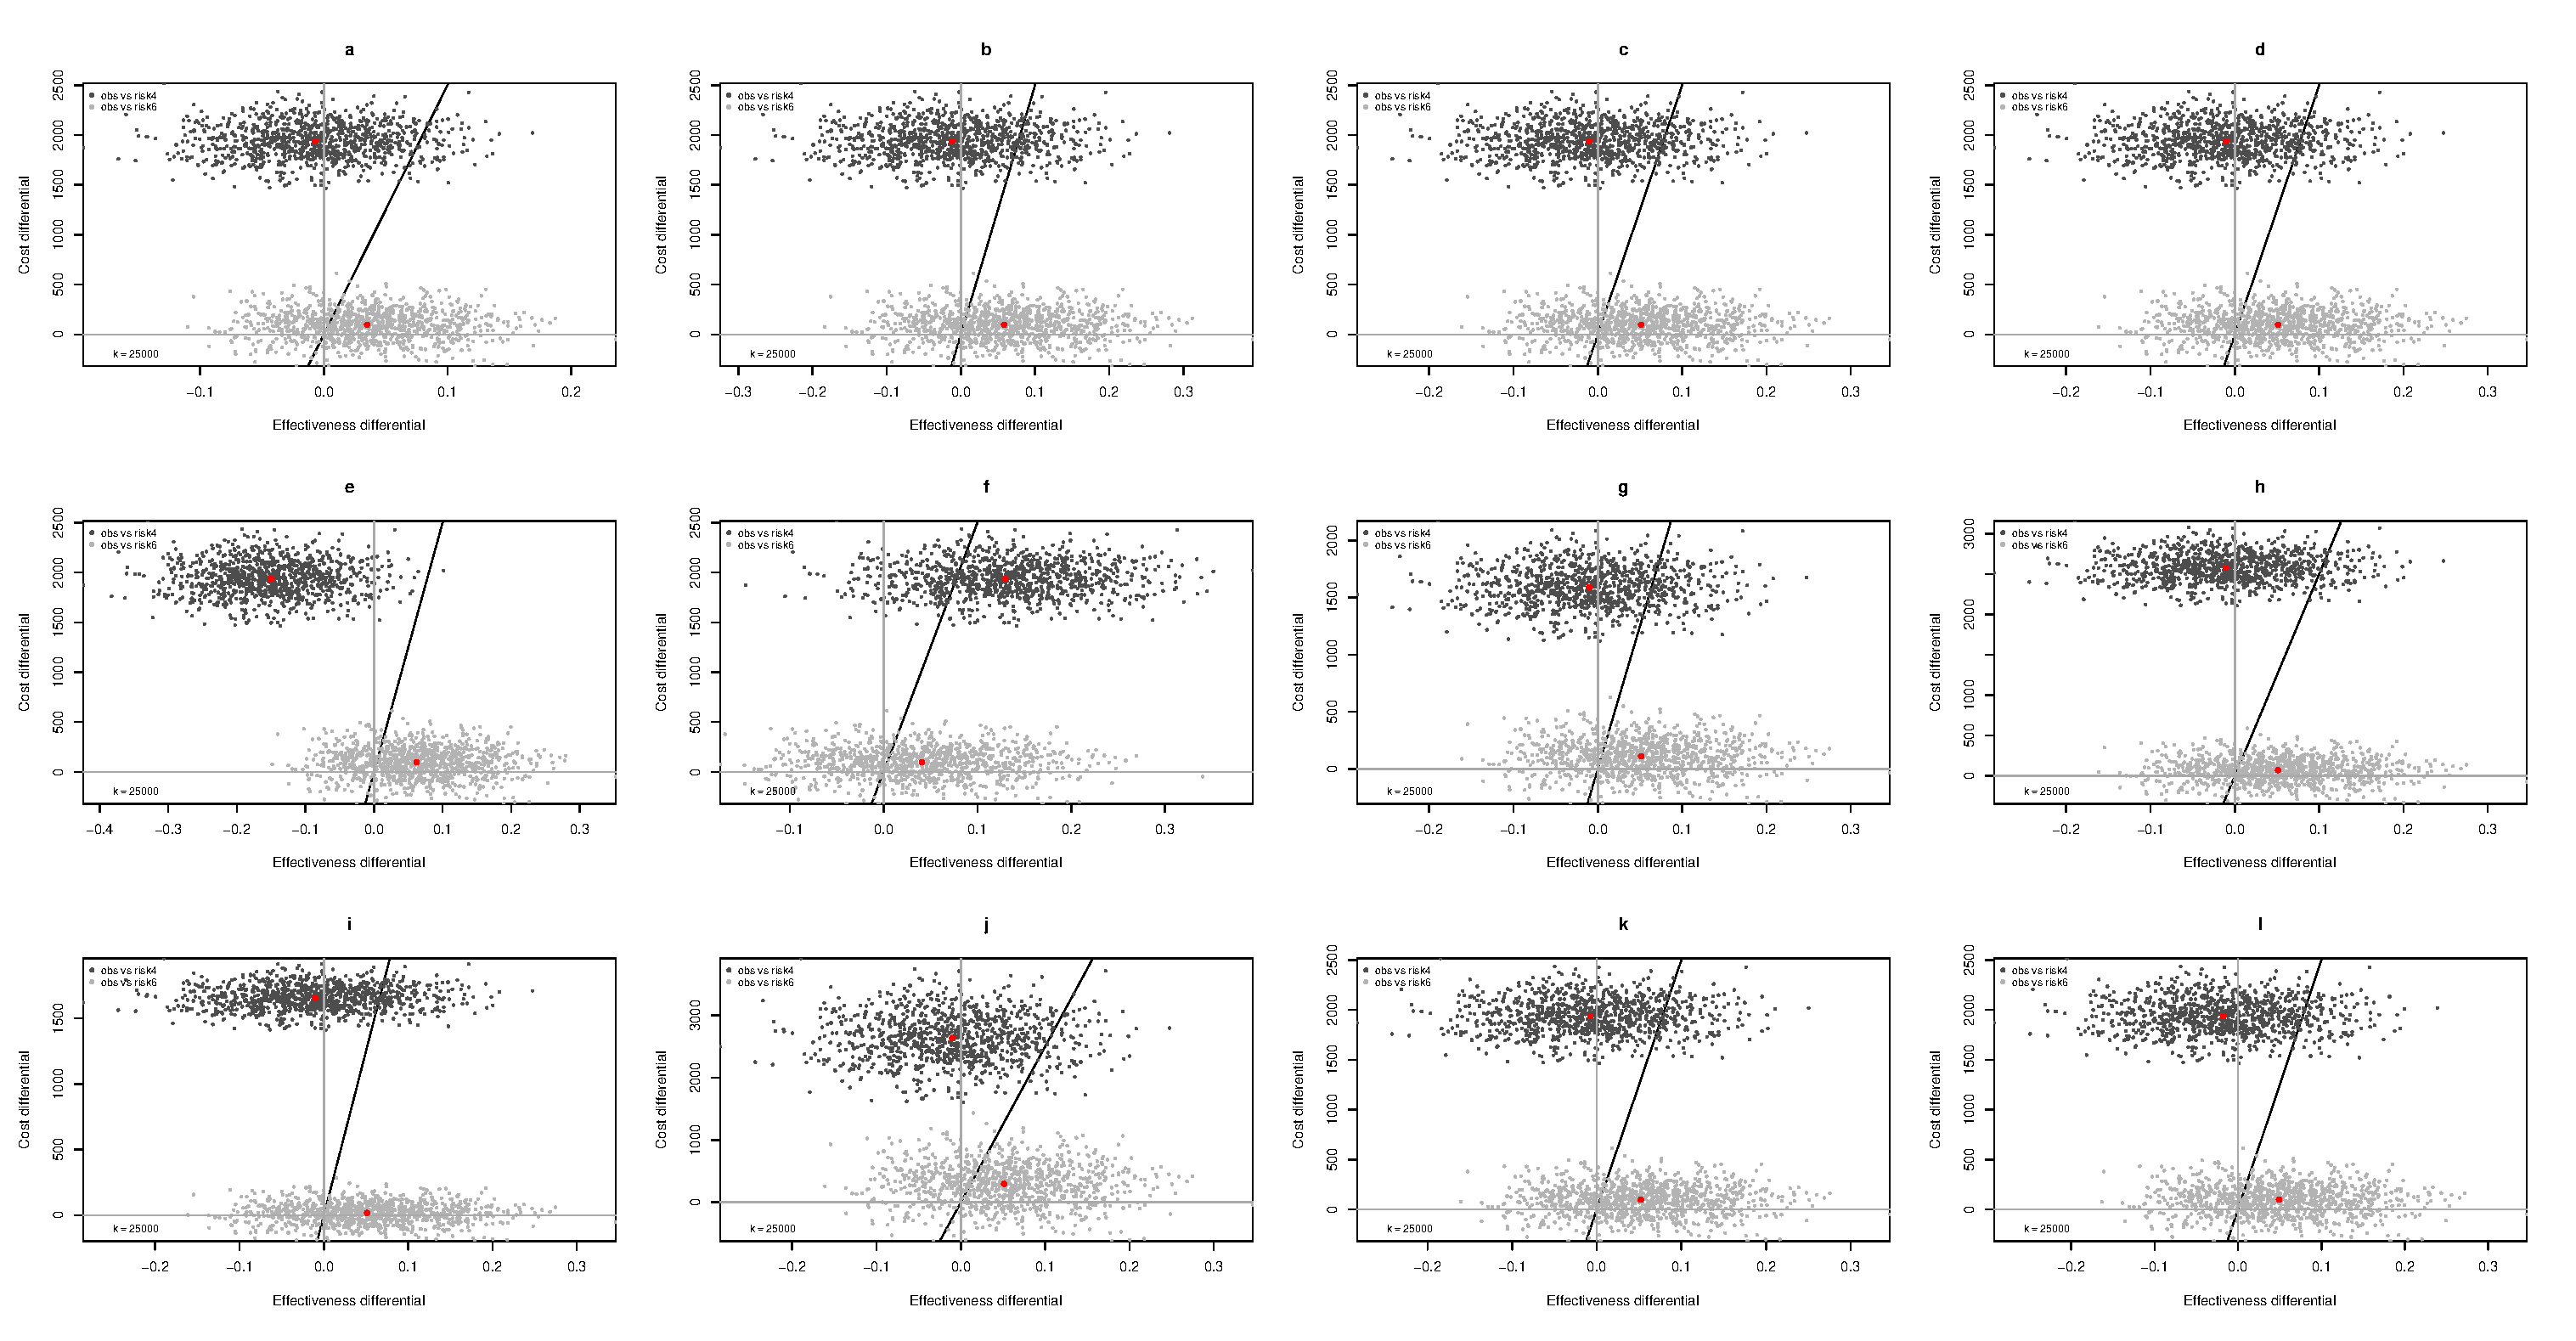
\includegraphics[width=0.6\linewidth]{../../images/ceplane_grid} 

}

\caption{Cost-effectiveness planes. Black points are the 6\% threshold Cox model and grey points are the 4\% threshold Cox model. Mean values are indicated in red and a willingness to pay threhold for £25,000 is indicated with the diagonal line.}\label{fig:ceplane}
\end{figure}

\hypertarget{discussion}{%
\subsection{Discussion}\label{discussion}}

Decision making as to whether to have the implant is shared between
patient and medical professional. The SCD risk score is a support tool
which contributes to the final decision. An SCD risk score of 6\%
provides a treatment recommendation for one patient versus another.
There could be individual preferences that out-weighs the risk score and
mean a patient chooses an alternative. Risk is viewed differently in
shared decision making between patients and clinicians (and also between
different clinicians).

collective decision-making is aided by CEAs but shaped by local data
-\textgreater{} price sensitive or QLY sensitive for each local
population. The main conundrum is that the tech offers delayed benefits
for the few and an initial upfront cost however the final decision to
implant is far more than a simple `economic calculation and much more
`value based'/ individual preferencing.

Having more robust quality of life data will help to make such
decisions. more embedded PROMs research within other projects and
systems.

Informatics Consult (Lai et al. 2021) automation to scale evidence
generation and to accelerate the return of results within clinical
time-scales.

We did not include CRT-D or s-ICD but that can be overcome by
sensitivity analyses that show e.g.~the main message is that conclusions
about the ICER etc will be robust to most departures from base
assumptions other than tweaks in utility (which are the part of the
model based on the weakest data!)

(Olivotto et al. 2020) The role of new DMARDs and their ability to
influence quality of life. So if both ICD and non-ICD patients
experience significant increases in QoL, are these equally distributed?

Although this paper is anticipate to be of most interest to an HTA
panel, the process of formally describing the development of the Markov
model over time, such as for example how many reimplantations and QoL
impact and unknowns etc that that could result in may in turn aid
decision making.

The nascent field of s-ICD in HCM would have a time horizons for battery
replacement lower than assumed for our analysis.

We could easily include the option of a fuzzy decision boundary such
that near the threshold there is some random variation as to whether a
patient received an ICD or not. Further this could formally incorporate
expert knowledge which would require an elicitation exercise.

\newpage

\hypertarget{references}{%
\section{References}\label{references}}

\hypertarget{refs}{}
\begin{CSLReferences}{1}{0}
\leavevmode\vadjust pre{\hypertarget{ref-Bryant2007}{}}%
Bryant, Jackie, Hakan Brodin, Emma Loveman, and Andrew Clegg. 2007.
{``{Clinical effectiveness and cost-effectiveness of implantable
cardioverter defibrillators for arrhythmias: A systematic review and
economic evaluation}.''} \emph{International Journal of Technology
Assessment in Health Care} 23 (1): 63--70.
\url{https://doi.org/10.1017/S0266462307051586}.

\leavevmode\vadjust pre{\hypertarget{ref-Buxton2006}{}}%
Buxton, M., N. Caine, D. Chase, D. Connelly, A. Grace, C. Jackson, J.
Parkes, and L. Sharples. 2006. {``A Review of the Evidence on the
Effects and Costs of Implantable Cardioverter Defibrillator Therapy in
Different Patient Groups, and the Modelling of Cost-Effectivenessan
Cost-Utility for These Groups in a UK Context.''} \emph{Health
Technology Assessment} 10 (27). \url{https://doi.org/10.3310/hta10270}.

\leavevmode\vadjust pre{\hypertarget{ref-Caro2007}{}}%
Caro, J. Jaime, Alexandra Ward, H. Baris Deniz, Judith A. O'Brien, and
Jenifer L. Ehreth. 2007. {``{Cost-benefit analysis of preventing sudden
cardiac deaths with an implantable cardioverter defibrillator versus
amiodarone}.''} \emph{Value in Health} 10 (1): 13--22.
\url{https://doi.org/10.1111/j.1524-4733.2006.00140.x}.

\leavevmode\vadjust pre{\hypertarget{ref-Colquitt2014}{}}%
Colquitt, Jill L, Diana Mendes, Andrew J Clegg, Petra Harris, Keith
Cooper, Joanna Picot, and Jackie Bryant. 2014. {``{Implantable
cardioverter defibrillators for the treatment of arrhythmias and cardiac
resynchronisation therapy for the treatment of heart failure: systematic
review and economic evaluation}.''} \emph{Health Technology Assessment}
18 (56). \url{https://doi.org/10.3310/hta18560}.

\leavevmode\vadjust pre{\hypertarget{ref-Cowie2009}{}}%
Cowie, Martin R., Deborah Marshall, Michael Drummond, Nicole Ferko,
Michael Maschio, Matthias Ekman, Luc de Roy, et al. 2009. {``Lifetime
Cost-Effectiveness of Prophylactic Implantation of a Cardioverter
Defibrillator in Patients with Reduced Left Ventricular Systolic
Function: Results of Markov Modelling in a European Population.''}
\emph{EP Europace} 11 (6): 716--26.
\url{https://doi.org/10.1093/europace/eup068}.

\leavevmode\vadjust pre{\hypertarget{ref-Cunningham2012}{}}%
Cunningham, David, Richard Charles, Morag Cunningham, and Adel de Lange.
2012. {``{National Audit of Cardiac Rhythm Management Devices 2012},''}
1--185.

\leavevmode\vadjust pre{\hypertarget{ref-Garcia-Perez2015}{}}%
García-Pérez, Lidia, Pilar Pinilla-Domínguez, Antonio García-Quintana,
Eduardo Caballero-Dorta, F. Javier García-García, Renata Linertová, and
Iñaki Imaz-Iglesia. 2015. {``{Economic evaluations of implantable
cardioverter defibrillators: a systematic review}.''} \emph{European
Journal of Health Economics} 16 (8): 879--93.
\url{https://doi.org/10.1007/s10198-014-0637-x}.

\leavevmode\vadjust pre{\hypertarget{ref-Holbrook2020}{}}%
Holbrook, Reece, Lucas Higuera, Kael Wherry, Dave Phay, Yu-Cheng Hsieh,
Kuo-Hung Lin, and Yen-Bin Liu. 2020. {``Implantable Cardioverter
Defibrillator Therapy Is Cost Effective for Primary Prevention Patients
in Taiwan: An Analysis from the Improve SCA Trial.''} \emph{PLOS ONE} 15
(11): e0241697. \url{https://doi.org/10.1371/journal.pone.0241697}.

\leavevmode\vadjust pre{\hypertarget{ref-Lai2021}{}}%
Lai, Alvina G, Wai Hoong Chang, Constantinos A Parisinos, Michail
Katsoulis, M Ruth, Anoop D Shah, Vincent Nguyen, et al. 2021. {``{An
Informatics Consult approach for generating clinical evidence for
treatment decisions}.''} \emph{medRxiv}.
https://doi.org/\url{https://doi.org/10.1101/2021.01.10.21249331}.

\leavevmode\vadjust pre{\hypertarget{ref-Lambiase2022}{}}%
Lambiase, Pier D, Dominic A Theuns, Francis Murgatroyd, Craig Barr, Lars
Eckardt, Petr Neuzil, Marcoen Scholten, et al. 2022. {``{Subcutaneous
implantable cardioverter- de fi brillators : long-term results of the
EFFORTLESS study},''} 1--14.

\leavevmode\vadjust pre{\hypertarget{ref-Lunn2000}{}}%
Lunn, D J, A Thomas, N Best, and David J. Spiegelhalter. 2000.
{``{WinBUGS -- a Bayesian modelling framework: concepts, structure, and
extensibility}.''} \emph{Statistics and Computing} 10: 325--37.

\leavevmode\vadjust pre{\hypertarget{ref-Magnusson2020}{}}%
Magnusson, Peter, and Anders Wimo. 2020. {``{Health economic evaluation
of implantable cardioverter defibrillators in hypertrophic
cardiomyopathy in adults}.''} \emph{International Journal of Cardiology}
311: 46--51. \url{https://doi.org/10.1016/j.ijcard.2020.02.055}.

\leavevmode\vadjust pre{\hypertarget{ref-Mealing2016}{}}%
Mealing, Stuart, Beth Woods, Neil Hawkins, Martin R. Cowie, Christopher
J. Plummer, William T. Abraham, John F. Beshai, Helmut Klein, and Mark
Sculpher. 2016. {``Cost-Effectiveness of Implantable Cardiac Devices in
Patients with Systolic Heart Failure.''} \emph{Heart} 102 (21):
1742--49. \url{https://doi.org/10.1136/heartjnl-2015-308883}.

\leavevmode\vadjust pre{\hypertarget{ref-Nauffal2021}{}}%
Nauffal, Victor, Peter Marstrand, Larry Han, Victoria N. Parikh, Adam S.
Helms, Jodie Ingles, Daniel Jacoby, et al. 2021. {``{Worldwide
differences in primary prevention implantable cardioverter defibrillator
utilization and outcomes in hypertrophic cardiomyopathy}.''} \emph{Eur.
Heart J.} 42 (38): 3932--44.
\url{https://doi.org/10.1093/eurheartj/ehab598}.

\leavevmode\vadjust pre{\hypertarget{ref-NHSEngland2021}{}}%
NHS England. 2021. {``{2021/22 National Tariff Payment System}.''}
\url{https://www.england.nhs.uk/publication/national-tariff-payment-system-documents-annexes-and-supporting-documents/}.

\leavevmode\vadjust pre{\hypertarget{ref-OMahony2014}{}}%
O'Mahony, Constantinos O, Fatima Jichi, Menelaos Pavlou, Lorenzo
Monserrat, Aristides Anastasakis, Claudio Rapezzi, Elena Biagini, et al.
2014. {``{Myocardial disease A novel clinical risk prediction model for
sudden cardiac death in hypertrophic cardiomyopathy (HCM Risk-SCD)}.''}
\emph{European Heart Journal} 35: 2010--20.
\url{https://doi.org/10.1093/eurheartj/eht439}.

\leavevmode\vadjust pre{\hypertarget{ref-Olivotto2020}{}}%
Olivotto, Iacopo, Artur Oreziak, Roberto Barriales-Villa, Theodore P.
Abraham, Ahmad Masri, Pablo Garcia-Pavia, Sara Saberi, et al. 2020.
{``Mavacamten for Treatment of Symptomatic Obstructive Hypertrophic
Cardiomyopathy (EXPLORER-HCM): A Randomised, Double-Blind,
Placebo-Controlled, Phase 3 Trial.''} \emph{The Lancet} 396 (10253):
759--69. \url{https://doi.org/10.1016/S0140-6736(20)31792-X}.

\leavevmode\vadjust pre{\hypertarget{ref-Ommen2020}{}}%
Ommen, Steve R., Seema Mital, Michael A. Burke, Sharlene M. Day, Anita
Deswal, Perry Elliott, Lauren L. Evanovich, et al. 2020. {``{2020
AHA/ACC Guideline for the Diagnosis and Treatment of Patients With
Hypertrophic Cardiomyopathy}.''} \emph{Circulation} 142 (25).
\url{https://doi.org/10.1161/cir.0000000000000937}.

\leavevmode\vadjust pre{\hypertarget{ref-R2021}{}}%
R Core Team. 2021. \emph{R: A Language and Environment for Statistical
Computing}. Vienna, Austria: R Foundation for Statistical Computing.
\url{https://www.R-project.org/}.

\leavevmode\vadjust pre{\hypertarget{ref-Sanders2005}{}}%
Sanders, Gillian D., Mark A. Hlatky, and Douglas K. Owens. 2005.
{``Cost-Effectiveness of Implantable Cardioverter--Defibrillators.''}
\emph{New England Journal of Medicine} 353 (14): 1471--80.
\url{https://doi.org/10.1056/NEJMsa051989}.

\leavevmode\vadjust pre{\hypertarget{ref-Smith2013}{}}%
Smith, T., L. Jordaens, D. A. M. J. Theuns, P. F. van Dessel, A. A.
Wilde, and M. G. M. Hunink. 2013. {``The Cost-Effectiveness of Primary
Prophylactic Implantable Defibrillator Therapy in Patients with
Ischaemic or Non-Ischaemic Heart Disease: A European Analysis.''}
\emph{European Heart Journal} 34 (3): 211--19.
\url{https://doi.org/10.1093/eurheartj/ehs090}.

\leavevmode\vadjust pre{\hypertarget{ref-Thijssen2014}{}}%
Thijssen, Joep, M. Elske van den Akker van Marle, C. Jan Willem
Borleffs, Johannes B. van Rees, Mihály K. de Bie, Enno T. van der Velde,
Lieselot van Erven, and Martin J. Schalij. 2014. {``Cost-Effectiveness
of Primary Prevention Implantable Cardioverter Defibrillator Treatment:
Data from a Large Clinical Registry.''} \emph{Pacing and Clinical
Electrophysiology: PACE} 37 (1): 25--34.
\url{https://doi.org/10.1111/pace.12238}.

\leavevmode\vadjust pre{\hypertarget{ref-Tomini2016}{}}%
Tomini, F. 2016. {``{A review of economic evaluation models for cardiac
resynchronization therapy with implantable cardioverter defibrillators
in patients with heart failure}.''} \emph{Eur J Health Econ}, 1159--72.
\url{https://doi.org/10.1007/s10198-015-0752-3}.

\leavevmode\vadjust pre{\hypertarget{ref-Yao2007}{}}%
Yao, Guiqing, Nick Freemantle, Melanie J Calvert, Stirling Bryan,
Jean-claude Daubert, and John G F Cleland. 2007. {``{The long-term
cost-effectiveness of cardiac resynchronization therapy with or without
an implantable cardioverter-defibrillator}.''} \emph{European Heart
Journal}, 42--51. \url{https://doi.org/10.1093/eurheartj/ehl382}.

\end{CSLReferences}

\newpage

\hypertarget{appendix}{%
\section{Appendix}\label{appendix}}

\hypertarget{health-and-cost-equations}{%
\subsection{Health and cost equations}\label{health-and-cost-equations}}

Subscript \(s\) denotes the state number and superscript denotes the
intervention either ICD or not.

\begin{itemize}
\item
  Annual health: \begin{align*} 
  e^i_{s=1}(t) &= q_{icd}, \;\; i = 1,2\\
  e^i_{s=3}(t) &= q_{hcm}, \;\; i = 1,2\\
  e^i_{s=2}(t) &= q_{hcm} - u_{shock}, \;\; i = 1,2\\
  e^i_{s}(t) &= 0, \;\;  i = 1,2, \; s = 4,5\\
  \end{align*}
\item
  Initial: \begin{align*}
  c^0_{s=1}(t = 0) &= c_{icd} + p_{compl} \times c_{compl}\\
  c^1_{s=1}(t = 0) &= c_{icd} + c_{rscore} + p_{compl} \times c_{compl}\\
  \end{align*} \emph{should we include this?} \[
  e^i_{s=1}(t = 0) = q_{hcm} - u_{implant} - p_{compl} \times u_{compl}, \;\; i = 1,2
  \]
\item
  Annual cost: \begin{align*}
  c^i_{s=1}(t) &= 2 c_{appt}, \;\;  i = 1,2,\\
  c^i_{s=2}(t) &= c_{shock},  \;\; i = 1,2\\
  \end{align*}
\end{itemize}

\hypertarget{bayesian-inference-of-transition-probabilities}{%
\subsection{Bayesian inference of transition
probabilities}\label{bayesian-inference-of-transition-probabilities}}

Denote \(x\) as the observed number of transitions, \(p\) the
probability of a transition and \(n\) as the total number of transitions
from a given state. The hyperparameters \(\alpha\) characterise the
prior knowledge on \(p\). Superscripts indicate the decision rule used.

\[x^{(1)}_{i.} \sim \mbox{Multinomial}(p^{(1)}_{i.}, n^{(1)}_i), \;\; i = 1,3\]

\[x^{(2)}_{i.} \sim \mbox{Multinomial}(p^{(2)}_{i.}, n^{(2)}_i), \;\; i = 1,3\]

\[p^{(1)}_{i.} \sim \mbox{Dirichlet}(\boldsymbol{\alpha}^{(1)} ), \;\; i = 1,3\]

\[p^{(2)}_{i.} \sim \mbox{Dirichlet}(\boldsymbol{\alpha}^{(2)} ), \;\; i = 1,3\]

For all sink states,

\[
p^{(s)}_{ij} = \left\{
\begin{array}{ll}
1 & \mbox{if $i = j$};\\
0 & \mbox{if $i \neq j$}.
\end{array} \right.
\]

\textbackslash begin\{figure\}

\includegraphics[width=0.5\linewidth]{../../images/init_hist_004}
\includegraphics[width=0.5\linewidth]{../../images/init_hist_006}
\hfill{}

\textbackslash caption\{Markov model initial HCM without ICD state
population histograms for 4\% and 6\% risk score threshold. The
uncertainty on the risk score model fit is propogated to the
stratification step. Red vertical lines indicate the sample averages
taking into account risk score model uncertainty and the blue vertical
lines indicate the point estimates direct from the data. The smoothed
densities are shown with the red curves.\}\label{fig:unnamed-chunk-5}
\textbackslash end\{figure\}

\end{document}
